%    Documentation for Irrigation Control Project
%    Copyright (C) 2017  Gregory Raven
%
%    This program is free software: you can redistribute it and/or modify
%    it under the terms of the GNU General Public License as published by
%    the Free Software Foundation, either version 3 of the License, or
%    (at your option) any later version.
%
%    This program is distributed in the hope that it will be useful,
%    but WITHOUT ANY WARRANTY; without even the implied warranty of
%    MERCHANTABILITY or FITNESS FOR A PARTICULAR PURPOSE.  See the
%    GNU General Public License for more details.
%
%    You should have received a copy of the GNU General Public License
%    along with this program.  If not, see <http://www.gnu.org/licenses/>.

\chapter{Running the Project}

\section{Cloning from Git and Installing Node Modules}

The project must be cloned to the BBGW and the NPM modules installed.

After ssh into the BBGW, typically you will be in directory /home/debian.
From there, enter these commands:

\begin{verbatim}
git clone https://github.com/Greg-R/irrigate-control.git
cd irrigate-control
cd software/node
npm install --save
\end{verbatim}

The project will be pulled from the git repository.  The node modules need to 
be installed in the directory from which the server will be launched.
The above should install the modules into a directory ``node\_modules''.

\section{Running the Irrigation Server}

Now it is time to run the server!

First, determine the IP address of the BBGW:

\begin{verbatim}
ip addr
\end{verbatim}

Look for the address associated with WLAN0 and remember it.  Next:

\begin{verbatim}
sudo node server.js
\end{verbatim}

If all goes well, the command line should look like this:

\begin{verbatim}
WebSocket server started...
Server is running at port 8089.
\end{verbatim}

Now open a brower, preferably Chromium or Chrome, and go to this URL:

\begin{verbatim}
http://192.168.1.3:8089/index_timer.html
\end{verbatim}

In this example, the IP address is: 192.168.1.3
The port number is 8089, and this is hard-coded into the server code.

You should get a web page like the following:

\begin{figure}[h]
	\centering
    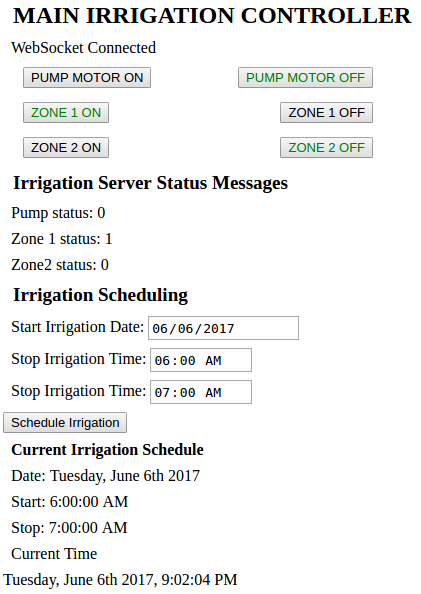
\includegraphics[width=0.5\textwidth]{photos/browser_full.png}
	\centering\bfseries
	\caption{The Irrigation Controller as seen with a Chromium Browser}
\end{figure}

The six buttons at the top toggle the three pump components on and off.  The 
left column is on, and the right column is off.  You should see the status 
display below the buttons updated as you click the buttons.

Setting the irrigation schedule is done by choosing clicking in the right hand 
end of the date form.  You will see the controls if you hover the mouse in that 
area.  Clicking on the triangular down arrow will bring up a calendar and the 
date can be chosen.

The start and stop input forms are set by clicking the hour minute and AM/PM 
fields in the form and then using the up/down arrows to set the desired time.

When the schedule is satisfactory, click the ``Schedule Irrigation'' button and 
a message will be sent to the server.  If all is well, the schedule is sent 
back to the browser and the ``Current Irrigation Schedule'' fields are updated.

The system will begin irrigation at the chosen date and time.  The time in 
zone1 and zone2 is divided in half based on the start and stop times.

The manual control buttons will still function during automated irrigation if 
it is desired to terminate watering early.

\section{Important Note on Closing the Web Browser}

It is important to properly close the web browser!

In order for WebSocket to properly close the connection, the ``tab'' from
which the irrigation web page is run must be closed.  If it is the only tab being used,
the create a new empty tab, and then close the irrigation tab.

If the entire brower is killed with the irrigation web page running, it is likely
that the WebSocket will not terminate correctly.  This has been observed to crash
the server.

Future updates will attempt to make this more robust.  It is believed that the periodic
time updates being sent via WebSocket from the server to the web browser make the
connection more fragile.  If this becomes a problem, comment out the line

\begin{verbatim}
        let timeDisplay = scheduler.timeDisplayUpdate();
\end{verbatim}

In the file websocketserver.js.

The computer local time can be used rather than the time broadcast from the server.
The disadvantage of this is that the time scheduling is done via the system time
of the server.  As long as this time is accurate, the irrigation will be timed accurately.








 
